\documentclass{article}
\usepackage[utf8]{inputenc}
\usepackage[T1]{fontenc}
\usepackage{graphicx}
\usepackage{hyperref}
\usepackage{geometry}
\geometry{margin=1in}

\title{781}
\date{Encyclopaedia Britannica (1771)}

\begin{document}
\maketitle

\section*{Historical source}
\textbf{Entry ID:} \texttt{entry-781-1017} \\
\textbf{Volume ID:} 144850367 \\
\textbf{Character Count:} 1908

\subsection*{Extracted Text}
the fixth for the pigans, and the feventh for the hy- pocrites of all religions.

Among Christians, there are two controverted quindices in regard to hell; is the one orchestra locality: the other the duration of its moments. The healthy of hell, and the reality of its fire, began frit to be controverted by Origen. That father, interpreted the freture account metaphorically, makes hell souffl not in external punilments, but in a confouficifa or fresh of guits, and a remainbame of poll pleasure. Among the modern, Mr YMillion advances a new hypothesis... According to him, the comets are farany hellis appointed in their orbits alternately to carry the channel into the cosmos of the fun, there to be forceful by its violent bars, and then to return with them beyond the orb of Saturn, there to flave them in their cold and difficult regions. Another modern author, not detailed with any hypothetical listeners advanced, alignes the fun to be the local hell.. As to the feecond quition, viz. the duration of both moments we have Origen again at the head of choice quite days that they are eternal; it being that father’s opinion, that not only men, but detaly, after a din course of punishment fortable to their respective critics, full be partained and refortered to heaven. The chief principle upon which Origen build his opinion, was the nature of punishment, which he took to be arcadency, applied only as phytic for the recovery of the patients' health. The chief objection to the certyly of heli torments among modern writers, is the disproportion between temporary crimes and extend punilments. Those who maintain the affirmative, ground their opinions on forture accounts, which expect the plans of fall under the figure of a worm which never dies, and a fire which is not quenched; as allo upon the words. "I Thief shall agree into overlifting punilment, but "to the rightness into like eternal.

\subsection*{Matched Wikipedia Article}
\textbf{Title:} Sikka Regency \\
\textbf{Page ID:} 3709808 \\
\textbf{Revision ID:} 1352263131 \\
\textbf{URL:} \url{https://en.wikipedia.org/wiki/Sikka\_Regency}


\section*{Source record}
\begin{itemize}
\item \textbf{Dataset:} \texttt{NationalLibraryOfScotland/encyclopaedia\_britannica\_illustrated}
\item \textbf{Dataset Revision:} \texttt{309f765b1ecc83e0a7f7762e44b4a927a7555443}
\item \textbf{Page ID:} \texttt{britannica:309f765b1ecc83e0a7f7762e44b4a927a7555443:train:1017} \\
  \textbf{Filename:} \texttt{page-1017-5395deb0e141.jpg} \\
  \textbf{Row Index:} 1017 \\
  \textbf{SHA256:} \texttt{5395deb0e1413694...}
\end{itemize}

\begin{figure}[h]
\centering
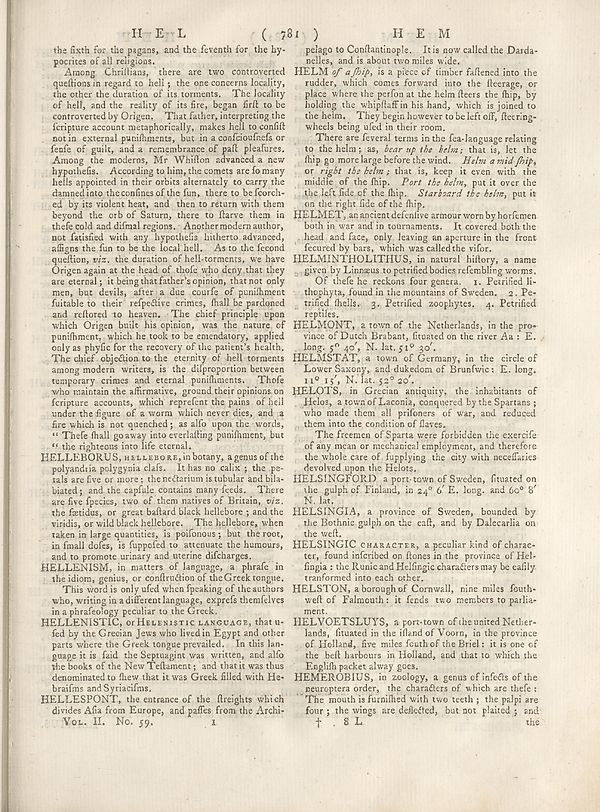
\includegraphics[width=0.85\textwidth]{../scans/page-1017-5395deb0e141.jpg}
\caption*{Source scan: \texttt{page-1017-5395deb0e141.jpg}}
\end{figure}

\end{document}
